\title{Simulazioni di Dinamica Molecolare}
\author{
        Antonio Michele Miti \\
                Department di Fisica \\
        Università Milano-Bicocca\\
        Piazza della Scienza 3, Milano 20126, \underline{Italy}
}
\date{\today}

% Formato pagina!
\documentclass[11pt]{article}
%\documentclass{acmconf}
\usepackage[paper=a4paper,dvips,top=1.5cm,left=1.5cm,right=1.5cm,
    foot=1cm,bottom=1.5cm]{geometry}

% Convenzioni Italiane
\usepackage[italian]{babel}



\usepackage{amsmath}

%Teoremi
\usepackage{amsthm}
\theoremstyle{plain}
\newtheorem{thm}{Teorema}[section]
\theoremstyle{remark}
\newtheorem{oss}{Osservazione}

%campi numerici
\usepackage{amsfonts}
\newcommand\Naturals{\ensuremath{\mathbb{N}}\xspace}
\newcommand\Integers{\ensuremath{\mathbb{Z}}\xspace}
\newcommand\Rationals{\ensuremath{\mathbb{Q}}\xspace}
\newcommand\Reals{\ensuremath{\mathbb{R}}\xspace}
\newcommand\Complex{\ensuremath{\mathbb{C}}\xspace}


%c C plus plus
\usepackage{relsize}
\usepackage{lipsum}
%c from texinfo.tex
\def\ifmonospace{\ifdim\fontdimen3\font=0pt }
\def\C++{%
\ifmonospace%
    C++%
\else%
    C\kern-.1667em\raise.30ex\hbox{\smaller{++}}%
\fi%
\spacefactor1000 }
%caratteri personalizzati per c++
\newcommand\Cls[1]{\textsf{#1}}
\newcommand\Lang[1]{\textsc{#1}}
\newcommand{\kw}[1]{\texttt{\textbf{#1}}}
\newcommand{\cd}[1]{\texttt{#1}}


%lettere accentate
\usepackage[utf8]{inputenc}


%usare immagini
\usepackage{graphicx}
\usepackage{latexsym}
\usepackage{wrapfig}
\usepackage{epstopdf}
\usepackage{caption}
\usepackage{subcaption}


%per visualizzare codice    http://texblog.org/2008/04/02/include-source-code-in-latex-with-listings/
\usepackage{listings}
\lstloadlanguages{ C++ }
\lstset{language=C++, numbers=left, stepnumber=2, frame=single,}

%Flow Chart
\usepackage{tikz}
\usetikzlibrary{shapes,arrows}
% Define block styles
\tikzstyle{decision} = [diamond, draw,aspect=1.8,text width=8em, text badly centered, node distance=3cm, inner sep=0pt]
\tikzstyle{block} = [rectangle, draw, 
    text width=13.5em, text centered, rounded corners, minimum height=5em]
\tikzstyle{block_largo} = [rectangle, draw, 
    text width=16.25cm, text centered, rounded corners, minimum height=4em]
\tikzstyle{block_med} = [rectangle, draw, 
    text width=12cm, text centered, rounded corners, minimum height=4em]    
\tikzstyle{line} = [draw, -latex']
\tikzstyle{cloud} = [draw, ellipse,fill=red!20, node distance=4.5cm,
    minimum height=2em]

%Diagrammi ad albero
\usetikzlibrary{trees,decorations.pathreplacing,decorations.pathmorphing}
\tikzstyle{casella} = [rectangle, draw, node distance=4.5cm,
    text width=20em]

%tabelle
\usepackage{multirow}


\begin{document}
\maketitle

\begin{abstract}
This is the paper's abstract \ldots
\end{abstract}

\tableofcontents
%/\/\/\/\/\/\/\/\/\/\/\/\/\/\/\/\/\/\/\/\/\/\/\/\/\/\/\/\/\/\/\/\/\/\/\/\/\/\/\/\/\/\/\
\section{Introduzione}\label{Introduzione}
Lo scopo delle simulazioni di Dinamica Molecolare è quello di dedurre le proprietà termodinamiche di un sistema fisico macroscopico in un punto specifico calcolando l'evoluzione dinamica dei sui componenti microscopi.
A questo scopo è necessario stabilire un modello della struttura microscopica che costituisce il sistema, ciò che nella scala macroscopica sarà solo un punto di un continuo corrisponderà ad una moltitudine di particelle fondamentali rispecchiandone le proprietà del loro moto collettivo. Tale punto viene detto  \emph{Punto Macroscopico} del sistema.

\begin{figure}
\centering
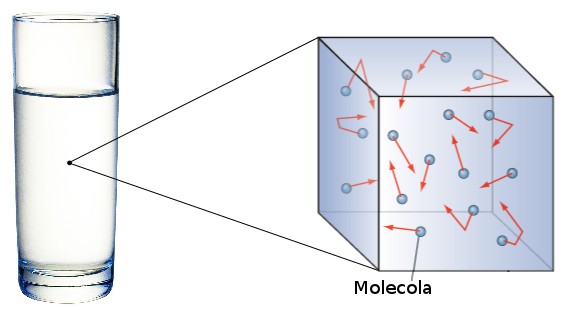
\includegraphics[scale=0.5]{Immagini/PuntoMacro.png}
\caption[Punto Macroscopico]{Punto Macroscopico}\label{fig: PuntoMacro}
\end{figure}

Un punto macroscopico di materiale continuo può essere modellizzato come una scatola cubica, di lato $L$ di estensione molto minore della dimensione lineare caratteristica del corpo, al cui interno sono contenute un numero $N$ (grande paragonabile al numero di Avogadro) di particelle, le molecole fondamentali costituenti l'oggetto.
In questo articolo si intendono studiare la dinamica molecolare classica, pertanto le particelle microscopiche saranno modellizzate come semplici punti materiali (\emph{Punti Microscopici}) sottostanti alle leggi della dinamica di Newton.

La scommessa della dinamica Molecolare è quella di dedurre lo stato macroscopico di un punto di un corpo continuo risolvendo la dinamica di un sistema microscopico opportunamente modellizzato.
La teoria fisica sottostante è molto semplice, il punto macroscopico è semplicemente un sistema classico  a molte particelle, la complicazione viene portata dal grande numero di sistemi elementari che vanno studiati complessivamente, in questo caso l'aiuto del calcolo computazionale diventa indispensabile. 

In conclusione il cuore di qualsiasi modello di Dinamica Molecolare classica sarnno gli algoritmi di simulazione della dinamica di sistemi a molte particelle.

\subsection{Dinamica dei sistemi a Molte Particelle}
I sistemi che verranno considerati saranno una collezione di $N$ punti materiali di massa $m$ in uno spazio $\mathbb{R}^d$.
La cinematica del sistema verrà specificata fornendo la descrizione dei vettori
\begin{displaymath}
\vec{\mathbf{R}}=(\vec{r_1},\ldots,\vec{r_N}) \qquad \vec{\mathbf{V}}=(\vec{v_1},\ldots,\vec{v_N}) \qquad \vec{\mathbf{A}}=(\vec{a_1},\ldots,\vec{a_N}) 
\end{displaymath}
in funzione del tempo.\newline
Il sistema verrà considerato isolato, le uniche interazioni saranno quelle esercitate reciprocamente dalle particelle costituenti. Le Forze verranno assunte conservative, la forma del potenziale corrispondende verrà considerata additiva e a due corpi (le interazioni a molti corpi verranno trascurate) pertanto l'equazione dell'energia interna del sistema assumerà la forma:
\begin{displaymath}
\mathcal{U}(\vec{\mathbf{R}}) = \sum\sum_{i>j}u(r_{ij})
\end{displaymath}
dove $u(r_{ij})$ è il potenziale di interazione tra due particelle poste a distanza scalare $r_ij = |\vec{r_i}-\vec{r_j}|$.
\newline
Come detto in precedenza la dinamica è classica, quindi la traiettoria di ogni particella dovrà soddisfare l'equazione di Newton:
\begin{displaymath}
\vec{F}_i = - \dfrac{\textrm{d}}{\textrm{d}\vec{r_i}} \Bigr(\sum_{j \neq i}u(r_{ij}) \Bigr) = m \cdot \vec{a_i}
\end{displaymath}
nel complesso l'evoluzione sarà regolata da un sistema di $N$ equazioni differenziali di questo tipo.
\newline
In un sistema isolato l'energia meccanica totale $ E = K + \mathcal{U} $ dovrà essere costantemente conservata. Inoltre ponendosi nel sistema di riferimento del centro di massa la forza totale $\vec{\mathbf{F}}$ e il momento totale $\vec{\mathbf{P}}$ dovranno risultare costantemente nulli.
\medskip\newline
Ciò che veramente interesserà determinare del sistema microscopico saranno le sue osservabili collettive che definiscono lo stato termodinamico del sistema nel suo complesso (si contrappongono alle variabili $(\vec{\mathbf{R}},\vec{\mathbf{V}}$ che invece fissano lo stato microscopico del sistema). \newline
Per un sistema di $N$ particelle contenute in volume $V=L^d$ si definiscono:

\begin{itemize}
\item \underline{Temperatura} $T$. Per il teorema di equipartizione dell'enegia risulta l'equazione:
\begin{equation}\label{eq: temperatura}
K = \dfrac{d}{2}N k T
\end{equation}
che definisce la temperatura istantanea della configurazione, il suo variabile osservabile sarà una media temporale su molte configurazioni.

\item \underline{Pressione} $P$. Dal tsonoeorema del viriale risulta l'equazione:
\begin{equation}\label{eq: Pressione}
Z = \dfrac{P V}{N kT} = 1 + \dfrac{1}{d N kT} \Biggr\langle \sum_{i=1}^N \vec{r_i}\cdot\vec{F_i}\Biggr\rangle
\end{equation}
dove $Z$ viene chiamato \emph{Fattore di comprimibilità} e con $\langle \cdot \rangle$ si intende la media temporale su molte configurazioni.

\item \underline{Densità} $\rho$. Definita come il rapporto tra la massa totale delle particelle e il volume che le contiene. In un sistema classico non sono previsti fenomeni di creazioni o deformazione dei gradi di libertà interni delle particelle, pertanto sarà una costante qua meno di scambi di materia del sistema con l'ambiente.
\end{itemize}
Queste osservabili saranno delle costanti del moto quando il sistema si trova in uno stato di equilibrio termodinamico.

\medskip
Ciò che distinguerà un modello di meccanica molecolare classica da un altro sarà la definizione della forma specifica del potenziale $u(r_{ij})$ di interazione a due corpi. Diriconoscono due classi di sistemi: quello dei corpi soffici, per cui le forze intermolecolari sono funzioni continue della distanza recipraca tra le due molecole, e quella dei corpi duri dotati di potenziali discontinui.






\subsection{Simulazione Computazionale dei sistemi a Molte Particelle}\label{cap: Simulazione in Generale}
Tutti gli algoritmi di simulazione di dinamica molecolare classica presentano degli aspetti comuni.
\begin{itemize}


\item \underline{Numero di Particelle e Limite Termodinamico}\newline
Se ci si aspetta che questi modelli descrivano il comportamento di una piccola porzione di un corpo continuo bisognerà considerare un numero di molecole paragonabile al numero di Avogadro ($N_A = 6,022 \cdot 10^23$), una quantità di variabili troppo grande per essere trattata in modo efficiente da un computer.

In una simulazione computazionale si è obbligati a considerare un numero molto minore di particelle da quelle richieste teoricamente, questo limite determina degli errori sistematici sui valori ottenuti rispetto al valore atteso degli osservabili nel punto del sistema macroscopico.

Questo vincolo di $N\ll N_A$ imposto dai limiti tecnici della simulazione non si può eliminare direttamente ma si può aggirare, ottenendo comunque una buona stima del valore d'aspattazione teorico, tramite un'estrapolazione dei dati.
\newline
Calcolando il valore d'aspettazione di un osservabile per numerosi sistemi nelle stesse condizioni termodinamiche (densità e temperatura) ma con numero di particelle diverso (sufficientemente grande da evitare situazioni patologiche per i potenziali ma limitato in modo da mantenere contenuto il tempo macchina necessario all'esecuzione) ed eseguendo un fit di tali dati in funzione di $N$ si potrà ottenere il valore atteso come il limite per $N\gg 1$ dell'andamento ottenuto (limite termodinamico).


\item \underline{Disposizione Iniziale delle particelle}\newline
Se lo scopo della simulazione del sistema a molte particelle è quello di simulare gli atomi costituenti un corpo macroscopico bisognerà imporre in ogni caso che la forma del potenziale sia repulsiva a corta distanza, ovvero che
\begin{displaymath}
u(r) \xrightarrow[r \rightarrow 0]{} \infty
\end{displaymath}
Un potenziale di questo tipo non permette di inizializzare il sistema con posizioni casuali, questa disposizione determinerebbe con frequenza stati in cui alcuni atomi sono molto vicini gli uni agli altri dando vita ad interazioni repulsive eccessivamente intense che distorcerebbero la dinamica del sistema.

La soluzione migliore per controllare questo problema è di disporre le posizioni iniziali delle particelle del sistema lungo un reticolo ordinato (solitamente \emph{Cubico a Corpo Centrato} o BCC), dopo un certo lasso di tempo detto \emph{termalizzazione}, l'azione continua delle interazioni porterà il sistema ad evolversi verso una configurazione più probabile.
	\begin{figure}[h!]
		\centering
		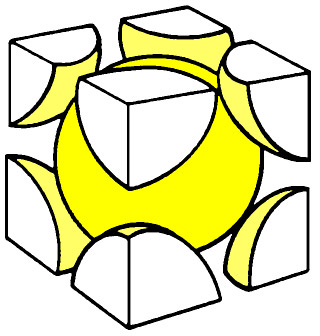
\includegraphics[scale=0.45]{Immagini/BCC.jpg}
		\caption[BCC]{Disposizione in reticolo BCC}\label{fig: BCC}
	\end{figure}


\item \underline{Inizializzazione delle velocità}\newline
Interessa studiare un punto del continuo macroscopico a riposo, quindi è naturale porsi in un sistema di riferimento solidale con il centro di massa delle $N$ particelle microscopiche.
In altre parole il momento totale del sistema deve essere nullo.

Per ottenere questa condizione è sufficiente inizializzare le componenti delle velocità di tutte le particelle in modo casuale , con $-1 < \vec{V}\cdot\hat{n} < 1$ ($\hat{n}$ versore di un asse del sistema cartesiano della "scatola"),e poi riscalare tutte le velocità in modo che il momento totale sia azzerato:
\begin{displaymath}
\vec{v_i} \longmapsto \vec{v_i}\cdot \dfrac{1}{\sum_{i}^{}\vec{v_i}}
\end{displaymath}


\item \underline{Condizione di Bordo Periodico}\newline
Per rappresentare un punto di un porzione continua di un materiale il sistema non può essere considerato una scatola immersa nel vuoto ma deve essere necessariamente circondato da sistemi dello stesso tipo posti a distanza trascurabile rispetto alla dimensione caratteristica del blocco di sostanza. 
Il sistema va quindi considerato confinato in una scatola cubica con altre scatole cubiche dello stesso tipo adiacenti ad ogni faccia, queste scatole modellizzano un insieme di punti macroscopici del materiale infinitamente vicini tra loro. 

Solitamente lo studio è finalizzato a studiare un punto del corpo in equilibrio termodinamico con l'intorno di materiale a lui vicino, quindi tutti gli altri sistemi adiacenti dovranno essere in uno stato microscopico simile al sistema considerato.
\newline
Questa condizione viene approssimata considerando tutti i sistemi adiacenti, in ogni direzione, nello stesso identico stato microscopico del sistema preso in esame. 

	\begin{figure}[h!]
		\centering
		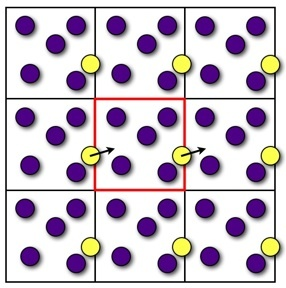
\includegraphics[scale=0.5]{Immagini/BordoPeriodo.jpg}
		\caption[Bordo Periodico]{Bordo Periodico e metodo delle immagini.}\label{fig: BordoPeriodo}
	\end{figure}

Pertanto quando si computeranno le interazioni esercitate su una particelle non si potranno considerare solo le interazioni con le altre particelle del sistema contenute nella scatola ma anche quella con tutte le altre nei sistemi limitrofi che saranno copie esatte delle particelle del sistema traslate di un unità di lato $L$.
(Quando si considerà questa approssimazione sarà necessario provvedere a "tagliare" la forma della funzione potenziale in modo da poter considerare nulla l'interazione ad una certa distanza).

Resta da considerare che la scatola contenente il sistema non può essere considerata infinita, in questo caso può capitare che una particella esca dalla scatola e entri nel volume adiacente.

La \underline{condizione di bordo periodico} è la soluzione ideale per tenere conto di questo scabio termodinamico tra sistemi identici, un bordo di questo tipo compensa l'uscita della particella da una parete dellla scatola con l'ingresso di una particella identica dalla faccia opposta della scatola.


\item \underline{Termalizzazione}\newline
All'inizializzazione la distribuzione delle componenti delle velocità sarà uniforme, ovvero i campioni delle velocità del sistema saranno egualmente distribuite in un intervallo prestabilito.
Lasciando evolvere naturalmente il sistema iniziale ordinato (in un reticolo BCC) per un intervallo di tempo sufficientemente grande il sistema si troverà in una configurazione ormai indipendente da quella inziale e soddiferà le ipotesi della distribuzione di \emph{Maxwell-Boltzman}.
In questo caso l'insieme di una determinata componente cartesiana delle velocità di tutte le particelle costituenti il sistema soddisferà una distribuzione gaussiana di questo tipo:
\begin{equation}
f(v_i) dv_i = \dfrac{1}{N} \: N(v_i) dv_i = \dfrac{1}{\mathcal{N}} \: e^{-A v_i^2} \qquad 
\textrm{dove} \; \mathcal{N} = \sqrt{\dfrac{\pi}{A}} \;\; \textrm{e} \;\; A = \dfrac{1}{2}\dfrac{m}{kT}
\end{equation}
qualsiasi sia la componenti $i$ considerata.


In un sistema con un numero $N$, finito e piccolo di particelle, non è possibile stimare una distribuzione continua, ma lo studio dell'istogramma normalizzato di questi valori è un buon criterio per determinare la corretta termalizzazione del sistema simulato. 
Per raffinare un grafico di questo tipo , oltre ad aumentare il numero di particelle della simulazione, si può incrementare la statistica raccolta accumulando velocità per diversi configurazioni a tempi successivi, se il sistema è effettivamente termalizzato i dati saranno compatibili e il sistema oscillerà tra configurazioni di equilibrio equiprobabili.

In alternativa si può valutare la funzione di Boltzman che associa ad ogni configurazione un valore definito da:
\begin{equation}
H_x = \int dv_x f(v_x) \ln{\biggr(f(v_x)\biggr)} = \sum_{\Delta v_x}^{}f(v_x) \ln{ \biggr(f(v_x)\biggr)} \Delta v_x
\end{equation} %=  - \dfrac{1 + \ln{(\mathcal{N}})}{2}
dove nell'ultima eguaglianza è data la versione per un sistema finito tramite integrazione per rettangoli dell'istogramma.
Quando la distribuzione presenta l'andamento gaussiano previsto risulterà:
\begin{equation}
H_i = \dfrac{1}{\mathcal{N}}\int dv_x \, e^{-A v_i^2} \, \ln{(\dfrac{e^{-A v_i^2}}{\mathcal{N}})} 
= \dfrac{-1}{\mathcal{N}} \Biggr( \int dv_x(A\, v_i^2)\, e^{-A v_i^2} + \ln{\mathcal{N}}\int dv_x e^{-A v_i^2}  \Biggr)
=- ( \dfrac{1}{2} + \ln{\mathcal{N}})
\end{equation}

Il discorso sull'aumento della statistica raccolta si applica anche in questo caso visto che l'integrale è calcolato sulla disribuzione discretizzata ovvero l'istogramma.


\item \underline{Grandezze Adimensionate}\newline
Il calcolatore può trattare solo numeri puri quindi in ogni simulazione computazionale è necessario stabilire delle unità dimensionali specifiche del sistema in modo da poter interpretare fisicamente i dati ottenuti dalla simulazione.
Un procedimento sicuro per ottenere un sistema di unità di misura classico completo è fissare tre unità tra MASSA LUNGHEZZA ENERGIA E TEMPO in modo da poter esprimere ogni altra grandezza derivata in funzione di esse.
La scelta verrà effettuata sfruttando i parametri dimensionali caratteristici di ogni specifica simulazione.


\item \underline{Studio delle Transizioni di Fase}\newline
Come già detto lo scopo di questo studio è di derivare il comportamento fisico macroscopico dei continui come manifestazione della struttura microscopica della materia.
Per un campione di materiale macroscopico si riconoscono almeno 3 stati fisici di aggregazione solido, liquido  e gassoso.
Ci si aspetta che una simulazione di dinamica molecolare ben definita possa simulare queste transizioni al variare delle variabili di stato pressione, volume e temperatura (sempre a seguito di una corretta termalizzazione).

Per semplicità si studia l'andamento di P in funzione di $\rho$ e T che sono variabili più facili da fissare durante l'inizializzazione del sistema, in tal caso si dice che la Pressione funge da parametro d'ordine del sistema.
Ci si aspetta quindi che una qualsiasi irregolarità o discontinuità dell'andamento del parametro d'ordine, incompatibilmentee con gli errori statistici sulla misura, possa essere sintomo di una transizione di fase del sistema.

Oltre al parametro d'ordine P è possibile studiare la diffussione per rilevare la fase in cui si trova il sistema.
La differenza principale che intercorre tra un sistema in fase solida e in fase fluida e la libertà di movimento delle molecole.
In un sistema solido  le particelle sono vincolate ad occupare una posizione prefisata in un reticolo potendo al limite oscillare attorno ad una posizione d'equilibrio.
Al contrario in un sistema liquido o gassoso le particelle sono libere di fluire nel volume, attraversarlo e in sufficiente tempo anche uscire da esso.

Per determinare qual'è il comportamento caratteristico di diffusione del sistema si possono misurare due osservabili.
La prima è lo \emph{spostamento quadratico medio} delle particelle :

\begin{equation}
\biggr\langle dS^2(t) \biggr\rangle = \biggr\langle\big\vert \vec{r_i}(t) - \vec{r_i}(0) \big\vert^2  \biggr\rangle
\end{equation}

dove la distanza è misurata senza applicare la condizione di bordo, seguendo quindi le particelle non loro moto libero di diffusione eventualmente anche fuori dal volume iniziale, mentre la media e calcolata su numerose coppie di configurazioni a distanza temporale $t$ e su tutte le particelle.
	\begin{figure}
		\centering
		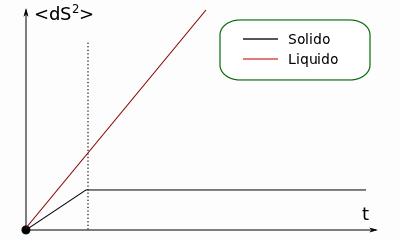
\includegraphics[scale=0.5]{Immagini/dS_quad_exp.png}
		\caption[Spostamento quadratico medio atteso]{Spostamento quadratico medio atteso}\label{fig: dS_quad_exp}
	\end{figure}
L'andamento atteso è mostrato nella figura \ref{fig: dS_quad_exp}, nella fase liquida le particelle propagheranno quasi linearmente diffondendo fuori dal volume, nella fase solida invece lo spostamente medio non potrà aumentare oltre il valore dell'oscillazione massima.

La seconda quantità che si può studiare è la \emph{funzione di distribuzione radiale} $g_t(r)$, ovvero la distribuzione dei valori dello distanza, calcolato con la condizione di bordo periodico, tra la posizione occupata da una particella al tempo $t_0=0$ e la posizione in cui si trova la stessa particella dopo un evoluzione temporale di $t$ del sistema. Ovvero, per un sistema finito, corrisponde all'istogramma dei valori di:
\begin{equation}
dS(t) = \big\vert \vec{r_i}(t) - \vec{r_i}(0) \big\vert
\end{equation}
campionati per diverse coppie di configurazioni a distanza temporale $t$ e per tutte le particelle.
\newline
Per un sistema solido si attende che la distribuzione $g_t(r)$ risulti molto piccata intorno ad un valore $r_o\ll D_{max}$(modulo dell'ampiezza di oscillazione) dove con $D_{max}$ si intende la massima distanza che si può estendere tra 2 punti in un sistema quadrato con condizioni di bordo periodico;
\begin{equation}
D_{max}= \frac{\sqrt{d}}{2}
\end{equation}
Mentre per un sistema fluido, se il tempo di evoluzione $t$ è sufficientemente alto, ci si aspetta che la distribuzione di probabilità di trovare la particella in punto specifico della scatola sia uniforme ovunque, ovvero dopo l'evoluzione la particella può trovarsi in ogni altro punto del volume in modo completamente casuale.
	\begin{figure}
		\centering
		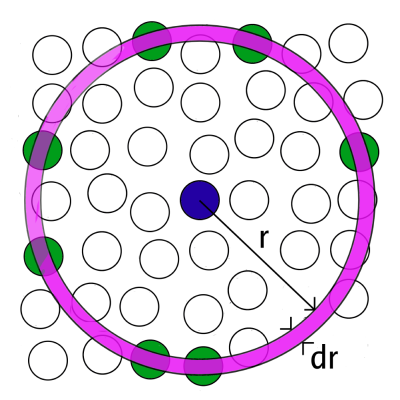
\includegraphics[scale=0.5]{Immagini/RDF.png}
		\caption[Funzione di Distribuzione Radiale]{ ---.}\label{fig: RDF}
	\end{figure}
In tal caso la distribuzione radiale crescerà in accordo con la crescita del volumetto elementare (figura \ref{fig: RDF}). Più precisamente se $\mathcal{\tilde{\rho}}(P)=\textrm{cost}$ è la distribuzione di probabilità (uniforme) di trovare la particella nel punto $P$ dopo l'evoluzione temporale, risulterà che:
\begin{eqnarray}
g_t(r) dr &=& \mathcal{\tilde{\rho}} \cdot 2\pi r\,dr   \qquad \textrm{(in 2 dimensioni)}    \nonumber \\
g_t(r) dr &=& \mathcal{\tilde{\rho}} \cdot \pi r^2\,dr   \qquad \textrm{(in 3 dimensioni)}    
\end{eqnarray}
almeno per distanze minori di $L/2$. 
Per distanze maggiori invece l'elemento di volume tende a decrescere all'aumentare della distanza, questo perchè sfere di raggio $L/2<r<D_{max}$ non possono essere completamente inscritte in un cubo di lato $L$, pertanto la distribuzione di probabilità tenderà a smorzarsi fino ad annullarsi a distanza $D_{max}$.
	\begin{figure}
		\centering
		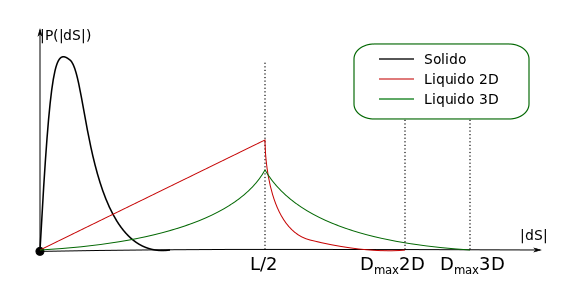
\includegraphics[scale=0.5]{Immagini/DistrodS.png}
		\caption[Distribuzione Radiale Attesa]{ ---.}\label{fig: DistrodS}
	\end{figure}
In conclusione isulterà un'andamento simile a quello mostrato nella figura (\ref{fig: DistrodS}).
% http://isaacs.sourceforge.net/phys/rdfs.html


\item \underline{Fasi Metastabili}\newline
In generale i sistemi considerati non mostreranno delle transizioni di fase nette, presenteranno invece delle \emph{Fasi metastabili} intorno ad alcuni caratteristici valori delle variabili di stato.
In questo tipo di stati si osserva che il parametro d'ordine oscillera in modo caotico tra le curve caratteristiche della fase precedente e della successiva.
Il motivo è che questo tipo di stati può assumere caratteristiche di entrambi le fasi, non perchè è una "via di mezzo" tra le due ma perchè può termalizzare in una qualsiasi delle due fasi a seconda delle condizioni iniziali.
In questa condizioni una piccola variazione dei parametri di stato può determinarare un netto cambiamento di fase, dimostrando un comportamento simile al caos deterministico della "mappa logistica".

\end{itemize}

Nei prossimi capitoli verrano applicate concretamente queste linee guida per studiare 2 modelli specifici di dinamica molecolare: il modello \emph{a "sfere dure"} e il modello \emph{a "sfere soffici"} con potenziale di \emph{ Lennard-Jones}.

\newpage
%/\/\/\/\/\/\/\/\/\/\/\/\/\/\/\/\/\/\/\/\/\/\/\/\/\/\/\/\/\/\/\/\/\/\/\/\/\/\/\/\/\/\/\
\section{Sfere Soffici}\label{Soffici}
In un generico modello a \emph{Sfere Soffici} il potenziale di interazione tra le particelle è una funzione continua della distanze.
\newline
Il potenziale più adatto alla descrizione delle interazioni intermolecolari è quello proposto su base fenomenologica da Lennard-Jones, definito dall'equazione:
\begin{equation}
u(r) = 4\epsilon \biggr[\big(\frac{\sigma}{r} \big)^{12} - \big(\frac{\sigma}{r} \big)^6 \biggr]
\end{equation}
dove la costante $\epsilon$ rappresenta il minimo dell'energia e $\sigma$ la distanza di annullamento del potenziale.
I due esponenti sono stati scelti attraverso un criterio empirico, devono essere tali da determinare una forza di attrazione tra particelle distanti e una bariera repulsiva a distanze piccole.
	\begin{figure}
		\centering
		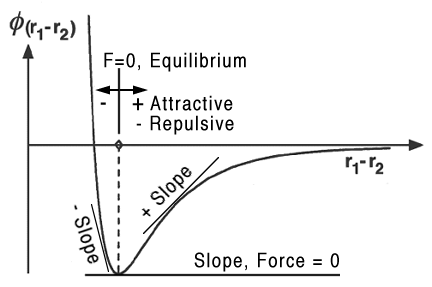
\includegraphics[scale=0.5]{Immagini/LJ}
		\caption[Potenziale di L.-J.]{Andamento del potenziale di Lennard-Jones.}\label{fig: LJunCut}
	\end{figure}




\clearpage
\subsection{Metodi Numerici e Simulazione Computazionale}
Come nel caso precedente, prima di passare allo studio del calcolo numerico della simulazione, è necessario scegliere un sistema di unità di misura caratteristico del modello.

\paragraph{Unità di Misura del sistema}
\begin{itemize}
\item[-] \underline{Massa}: $[M]=m=1$ 
\newline Tutte le particelle sono identiche è la loro massa fornisce l'unità di misura più ovvia.

\item[-] \underline{Lunghezza}: $[L]=\sigma=1$ 
\newline Il lato della scatola verrà quindi misurato in unità di $\sigma$ (diametro della scatola).

\item[-] \underline{Energia}: $[E]=\epsilon=1$ 
\newline Nell'espressione del potenziale è presente una scala naturale di energia data dalla costante $\epsilon$.
\end{itemize}

\subsubsection{Taglio del potenziale}
Per simulare l'evoluzione del sistema è necessario conoscere la forza totale applicata su ogni particella che lo compone.
L'interazione tra sfere soffici è a 2 corpi e a lungo range, pertanto di principio sarà necessario calcolare il contributo di interazione generato da ogni coppia di particelle, $N(N-1)$ contributi in totale.
Come è visibile dalla figura (\ref{fig: LJunCut}, la forza diventa rapidamente molto piccola al crescere della distanza, si può quindi avere un notevole aumento nell'efficienza dek calcolo trascuranto le interazioni che avvengono a grande distanza una distanza, quindi considerando un potenziale del tipo:
\begin{displaymath}
	u_c(r) = 
	\begin{cases}u(r) & r \leq r_c\\
	0 & r > r_c \end{cases}
\end{displaymath}
Un potenziale troncato in questo modo determina un simile troncamento anche per la funzione a lui corrispondente.
Questo taglio ha l'effetto di imprimere  dei piccoli impulsi ogni volta che una particella supera la distanza $r_c$ determinando delle oscillazioni nell'energia totale in contrasto con la conservazione prevista per un sistema isolato.
Per arginare questo effetto si definisce una nuova espressione approssimata per la forza d'interazione (troncata e traslata) definita dall'equazione:
\begin{equation}\label{eq: forza usata}
	F_{s}(r) = 
	\begin{cases}
	 -\dfrac{d}{dr} u(r) - \biggr(\dfrac{d}{dr} u(r)\biggr)\Biggr\vert_{r_c} & r \leq r_c\\
	0 & r > r_c 
	\end{cases}
\end{equation}
che determina un potenziale del tipo:
\begin{equation}\label{eq: potenziale usato}
	u_{s}(r) = 
	\begin{cases} u(r) - u(r_c) -[r -r_c]\biggr(\dfrac{d}{dr} u(r)\biggr)\Biggr\vert_{r_c} & r \leq r_c\\
	0 & r > r_c \end{cases}
\end{equation}
L'andamento delle nuove espressioni della forza e dell'interazione è visibile nella figura (\ref{fig: LJCut}), dal grafico si può vedere come la nuova forma alterata non sia estremamente dissimile dall'espressione iniziale.
	\begin{figure}
		\centering
		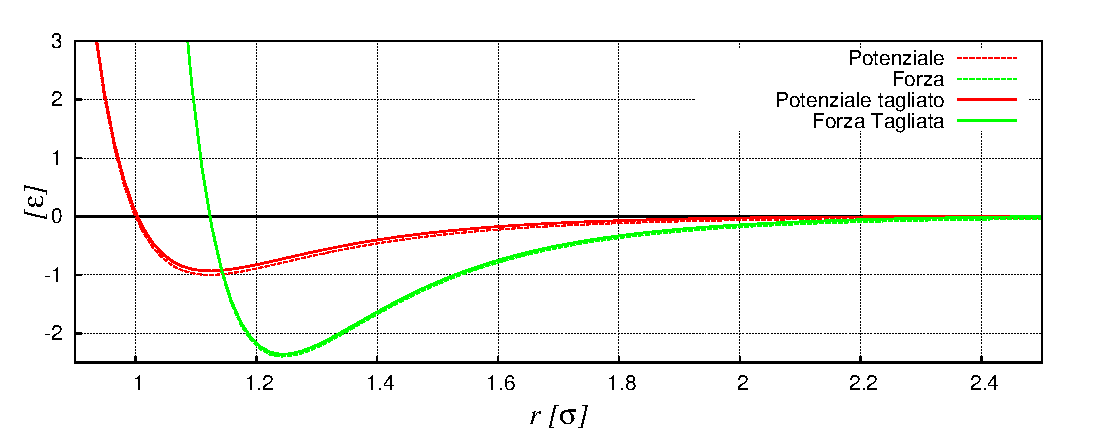
\includegraphics[scale=0.5]{Immagini/Soffici/potenziale}
		\caption[Potenziale di L.-J. tagliato]{Andamento del potenziale di Lennard-Jones tagliato e traslato e della forza corrispondente.}\label{fig: LJCut}
	\end{figure}
Tipicamente si sceglie come valore di taglio la distanza $r_c = 2.5 \sigma$ che corrisponde a trascurare valori della forza dell'ordine di $F(r_c) = -0.039 \epsilon / \sigma$.

\subsubsection{Metodo della lista dei vicini}
La parte della dinamica che richiede il maggiore sforzo computazionale è il calcolo della forza d'interazione, il metodo del potenziale troncato permette di migliorare l'efficienza di questa fase ma richiede in ogni caso di calcolare la distanza tra tutte le possibile coppie di particelle in ogni istante dell'evoluzione ( e in un sistema con bordo periodico tale misura non è immediata).

La velocità del calcolo numerico del sistema può essere ulteriormente raffinata introducendo la lista dei vicini.
Questa lista tiene conto di tutte le coppie di particelle che distano tra loro meno di $r_L \simeq r_c +0.3\sigma$, in questo modo funge da guida per indicare quali coppie di particelle sono sufficientemente vicine da determinare una forza d'interazione non trascurabile.
La distanza $r_L$ di "vicinanza" scelta è maggiore della distanza $r_c$ di "taglio", in questo modo la lista tiene traccia non solo delle particelle a distanza sufficientemente piccola da determinare un'interazione ma anche le particelle che entreranno nel raggio d'interazione in un certo intervallo di tempo $\check{T}$. In virtù di questa prescrizione non sarà necessario aggiornare la lista( e calcolare le distanze) ad ogni passo istante ma basterà farlo ogni $\check{T}$, intervallo di tempo pari a :
\begin{displaymath}
\check{T} \cdot \langle \vert \vec{v} \vert \rangle \simeq r_L - r_c = 0.3 \sigma
\end{displaymath}
corrispondende al tempo medio necessario ad una particella per percorrere la distanza $r_L - r_c$.

\subsubsection{Algoritmo di Evoluzione del sistema}
Nonostante queste modifiche alla forma matematica dell'interazione l'evoluzione dinamica del sistema risulta in ogni caso regolata dall'equazioni differenziali del moto.
Per un sistema dotato di un grande numero di particelle come quello in esame la soluzione esatta del sistema di equazioni di Newton è totalmente improponibile.
L'unico approccio possibile è quello di affidarsi alle soluzione approssimate fornite dai metodi del calcolo numerico.

Esistono diversi metodi per calcolare le soluzioni di equazioni differenziali in modo approssimativo, in generale nessuno di essi è in grado di calcolarla nel complesso ma solo di fornire una soluzione punto per punto risolvendo il problema di Cauchy per intervalli discreti consecutivi.

Nel seguito il tempo d'evoluzione verrà suddiviso in passi discreti pari a $t_{step} = 0.001 [t]$.


In questo articolo è stato sfruttato il metodo di \emph{Velocity Verlet} per la soluzione dell'equazione del moto che  implementato insieme alla tecnica della lista dei vicini determina il seguente algoritmo per il calcolo di un passo d'evoluzione del sistema:

\begin{figure}[h!]
\begin{tikzpicture}[node distance = auto]
    % Place nodes
    \node [block_med] (1) {Evoluzione delle posizioni di ogni particella di un passo $\Delta t = t_{step}$ \newline \footnotesize $$\vec{r_i}(t_0) \mapsto \vec{r_i}(t_0 + \Delta t) = \vec{r_i}(t_0) + \vec{v_i}(t_0) \cdot \Delta t + \dfrac{1}{2} \vec{a_i}(t_0) \cdot \Delta t^2$$};
    \node [block_med, below of=1,node distance=2.25cm] (2) {Calcolo delle velocità a mezzo passo. \newline \footnotesize $$ \vec{v_i}(t_0 + \Delta t/2) = \vec{v_i}(t_0) + \dfrac{1}{2} \vec{a_i}(t_0) \cdot \Delta t$$ };
    \node [block_med, below of=2,node distance=2.55cm] (3) {Ricalcolo delle accelerazioni delle particelle. \newline \footnotesize $$\vec{a_i}(t_0) \mapsto \vec{a_i}(t_0 + \Delta t)=
     \overbrace{\sum_{i}^{} \sum_{j>i}^{}}^{j \in \text{Vicini}(i)} 
     F_s(\bar\vec{r_i}(t_0 + \Delta t) -\vec{r_j}(t_0 + \Delta t \bar )$$}; %\textrm($j$ vicino a $i$)    
    \node [decision, right of=3,node distance=9.25cm] (5) {\footnotesize Riaggiornamento della lista dei vicini ogni $10$ passi $\Delta t$.};        
    \node [block_med, below of=3,node distance=2.75cm] (4) {Evoluzione delle velocità in accordo con le accelerazioni aggiornate \newline \footnotesize $$\vec{v_i}(t_0) \mapsto \vec{v_i}(t_0 + \Delta t) = \vec{v_i}(t_0 + \Delta t/2) + \dfrac{1}{2}\vec{a_i}(t_0+\Delta t)\cdot \Delta t$$};
 
    % Draw edges
    \path [line] (1) -- (2);
    \path [line] (2) -- (3);
    \path [line] (3) -- (4);
    \path [line] (4) -| (5);
    \path [line] (5) |- (1);
\end{tikzpicture}
\end{figure}


\clearpage
\subsubsection{Implementazione computazionale dell'algoritmo}
Per simulare questo sistema verrà utilizzata la programmazione ad oggetti del linguaggio C++.
La logica usata per il programma è la stessa sfrutta per la simulazione del sistema a sfere rigide.
\newline
Si definire la classe \Cls{sistema\_soffice()} dotata degli attributi necessari a descrivere lo stato microscopico del sistema:
\begin{itemize}
\item 3 array di vettori per memorizzare posizione, velocità e accelerazione di tutte le particelle costituenti il sistema.

\item 2 array per memorizzare la \emph{lista dei vicini} associata allo stato del sistema. Il vettore \cd{NPoint} contiene nell'ingresso $i$ l'indice del vettore \cd{List} dopo di cui comincia l'elenco delle particelle vicine alla particella $i$. Il vettore \cd{List} viene costruito testando in modo sequenziale tutte le coppie $($ $P[i]$, $P[j]$ $)_{j>i}$ e salvando tutti gli indici $j$ relativi a coppie "vicine" secondo la definizione del paragrafo precedente.

\item 5 variabili \emph{double} per contenere le variabili $r_c$, $r_L$,$\sigma$,$\epsilon$ e L. 2 varibili \emph{int} per salvare il numero di particelle e la dimensione spaziale della simulazione.

\end{itemize}
%\medskip\newline
Il costruttore della classe costituirà la fase di \emph{inizializzazione} dell'algoritmo, ovvero salverà le posizioni disponendole nel reticolo bcc più piccolo in grando di contenerle tutte, attribuirà velocità iniziali casuali riscalandole a Momento totale nullo, inizializza la lista dei vicini e calcola le accelerazioni per la prima volta.
Le variabili necessarie per inizializzare il sistema, argomenti della funzione costruttore, saranno la dimensione spaziale $d$, la densità del sistema e il numero $N$ di particelle contenute.
\medskip\newline
Il metodo \cd{evoluzione()} è il cardine della simulazione, questa funzione fornisce l'evoluzione temporale del sistema di un $t_{step}$ sfruttando la tavola dei vicini precedentemente calcolata. I metodi che calcolano passi d'evoluzione consecutivi provvederanno a ricalcolare la lista dei vicini ogni 10 $t_{step}$
\medskip\newline
La fase di \emph{termalizzazione} si ottiene applicando il metodo di evoluzione un numero di volte sufficiente a realizzare la distribuzione di Maxwell-Boltzman per le velocità.
\medskip\newline
Similmente la fase di \emph{produzione} si realizza intervallando la raccolta di osservabili istantanei sulla configurazione occupata dal sistema all'evoluzione temporale necessaria per ottenere un'altra configurazione sufficientemente scorrelata dalla prima.
\medskip\newline
Per ottenere rapidamente una successione di sistemi inizializzati con un diverso numero di particelle e valore di densità viene usato il metodo \cd{rinizializzazione()}. Tale metodo prende in ingresso i nuovi valore di $N$ e di $rho$ (minori di quelli precedenti), ricalcola il lato della scatola, espande proporzionalmente i vettori posizione e ricalcola la lista dei vicini di conseguenza.



\clearpage
\subsection{Caratteristiche dell'algoritmo di Simulazione}
\begin{figure}
		\caption[Sfere Soffici$/$Preliminari\_Snap2D.cpp]{Immagini del sistema 2D termalizzato a diversi valori di densità e Temperatura (In alto a sinistra è visibile la configurazione inziale prima dell'evoluzione temporale).}
        \begin{subfigure}[b]{0.5\textwidth}
                \centering
                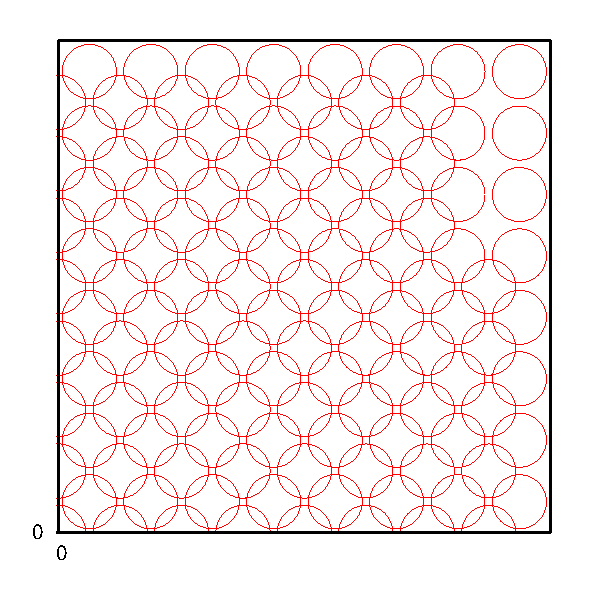
\includegraphics[width=0.85\textwidth]{Immagini/Soffici/SnapSolidoCompresso_Inizio_2D}
        \end{subfigure}%
        ~ %add desired spacing between images, e. g. ~, \quad, \qquad etc. 
          %(or a blank line to force the subfigure onto a new line)
        \begin{subfigure}[b]{0.5\textwidth}
                \centering
                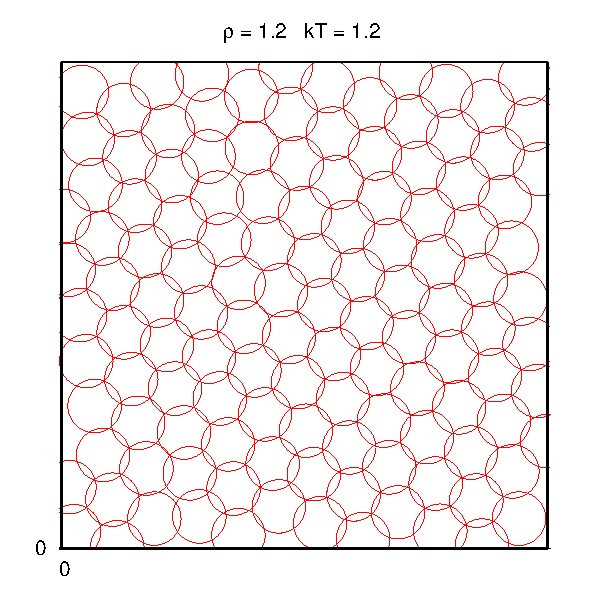
\includegraphics[width=0.85\textwidth]{Immagini/Soffici/SnapSolidoCompresso_2D}
        \end{subfigure}
        ~ %add desired spacing between images, e. g. ~, \quad, \qquad etc. 
          %(or a blank line to force the subfigure onto a new line)

        \begin{subfigure}[b]{0.5\textwidth}
                \centering
                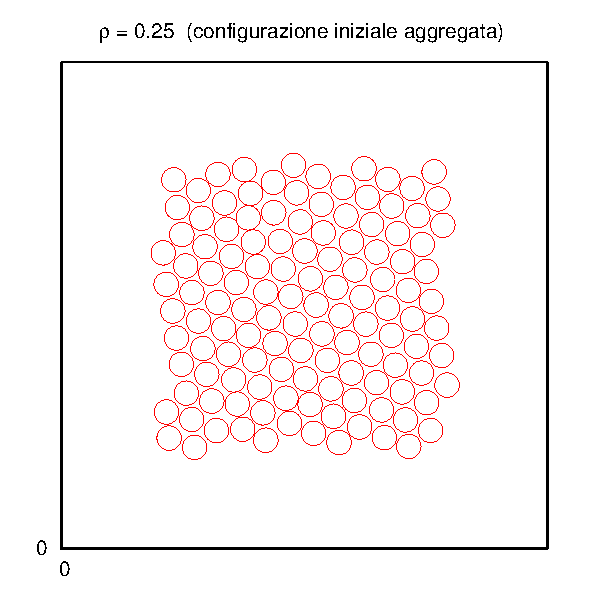
\includegraphics[width=0.85\textwidth]{Immagini/Soffici/SnapSolidoFreddo_Inizio_2D}
        \end{subfigure}
         \begin{subfigure}[b]{0.5\textwidth}
                \centering
                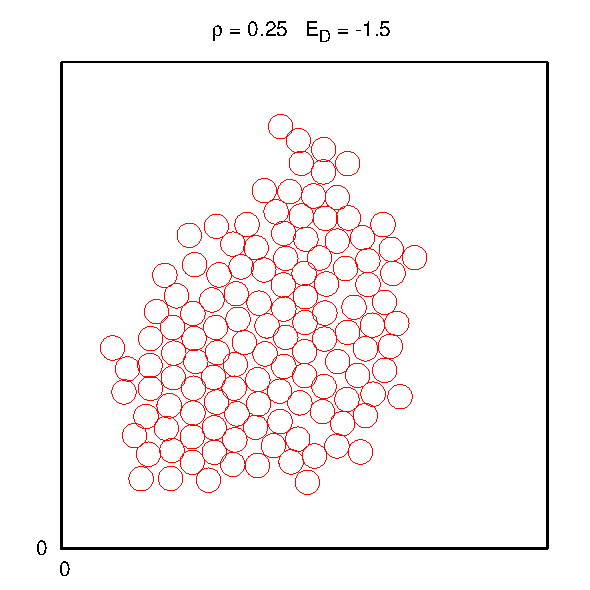
\includegraphics[width=0.85\textwidth]{Immagini/Soffici/SnapSolidoFreddo_2D}
        \end{subfigure}
		
        \begin{subfigure}[b]{0.5\textwidth}
                \centering
                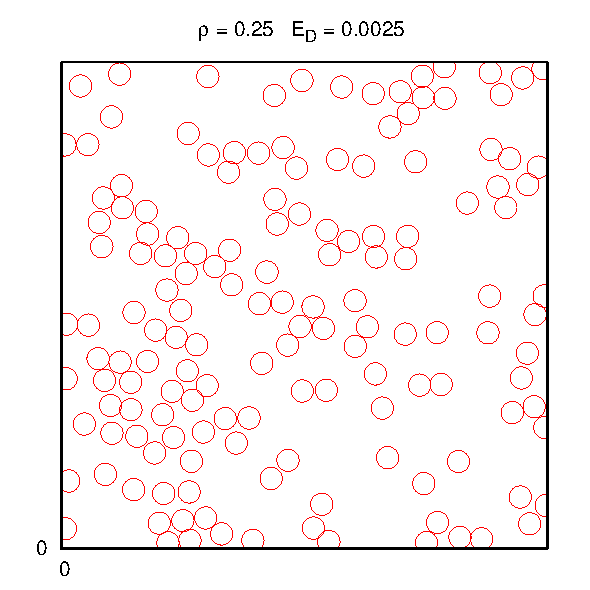
\includegraphics[width=0.85\textwidth]{Immagini/Soffici/SnapSolidoFreddo_2D_Nuclea}
        \end{subfigure}
         \begin{subfigure}[b]{0.5\textwidth}
                \centering
                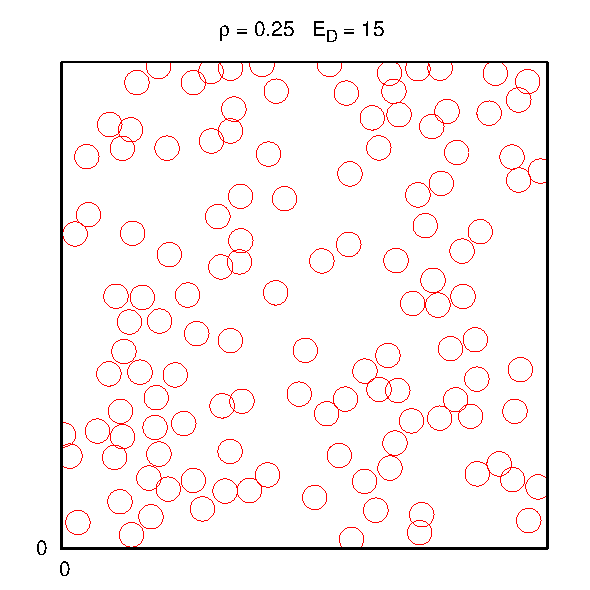
\includegraphics[width=0.85\textwidth]{Immagini/Soffici/SnapLiquido_2D}
        \end{subfigure}
		
		 \centering  \footnotesize{$N= 125$ , $d=2$ , N passi Termalizzazione =$ 500000 $}
		\label{fig: snap2d_soft}
\end{figure}
Nella figura (\ref{fig: snap2d_soft}) sono mostrate delle istantantanee delle configurazioni del sistema a sfere soffici termalizzato a diversi valori delle variabili Termodinamiche che certificano la presenza di una transizione di fase solido-liquido anche per questo modello.
Similmente a quanto accadeva per le sfere rigide il sistema presenta un congelamento di natura geometrica infatti per elevati valori di densità le molecole sono vincolate in un reticolo regolare per via della divergenza infinita del potenziale a brevi distanze.

Se l'energia media delle particelle è sufficientemente bassa, la presenza di forze attrattive determina la solidificazione del sistema anche in condizioni di bassa densità.
L'algoritmo usato per la termalizzazione, che consiste in una successione di passi evolutivi intervallati dal riscalamento delle velocità del sistema ad un valore di temperatura controllato, non è il procedimento ideale per mostrare questo tipo di transizione.
Nel caso in cui si cerchi di far solidificare un sistema molto rarefatto saranno necessari numerosi passi evolutivi affinchè le particelle, estremamente rallentate dall'abbassamento di temperatura, riescano ad avvicinarsi a sufficienza da aggregarsi e dare il via alla nucleazione.

L'immagine ottenuta precedentemente invece è stata realizzata a partire da una configurazione ordinata posta in un volume ampio( in modo da diminuire la densità totale), non è in grado di mostrare la solidificazione ma dimostra come il sistema rimanga aggregato in un regione densa in condizione di bassa temperatura sofficiente da non permettere alle molecole di fuoriuscire dai pozzi di potenziale generati dalla sovrapposizione di tutte le interazioni.
La simulazione riesce però a mostrare corrattamente l'evaporazione di questa struttura densa con il riscaldamento del sistema.

\subsubsection{Tempo di esecuzione}
Il parametro principale che regola il tempo macchina richiesto dalla simulazione di un singolo step di evoluzione del sistema è la lunghezza della lista dei vicini che principalmente dipende da 3 parametri della simulazione, il numero $N$ di particelle, la densità del sistema $\rho$ e la dimensione spaziale $d$.
Nella figura (\ref{fig: T_Esec Soffici}) è mostrato l'andamento del tempo di esecuzione medio di uno step evolutivo in fuzione del numero $N$ di particelle simulate e per vari valori di densità $\rho$.

	\begin{figure}
		\centering
		\caption[Sfere Soffici$/$Preliminari\_TempoEsecuzione.cpp]{Andamento del tempo di esecuzione in funzione del numero di particelle simulate e della Dimensione Spaziale.}\label{fig: T_Esec_Confronto_D Soffici}
		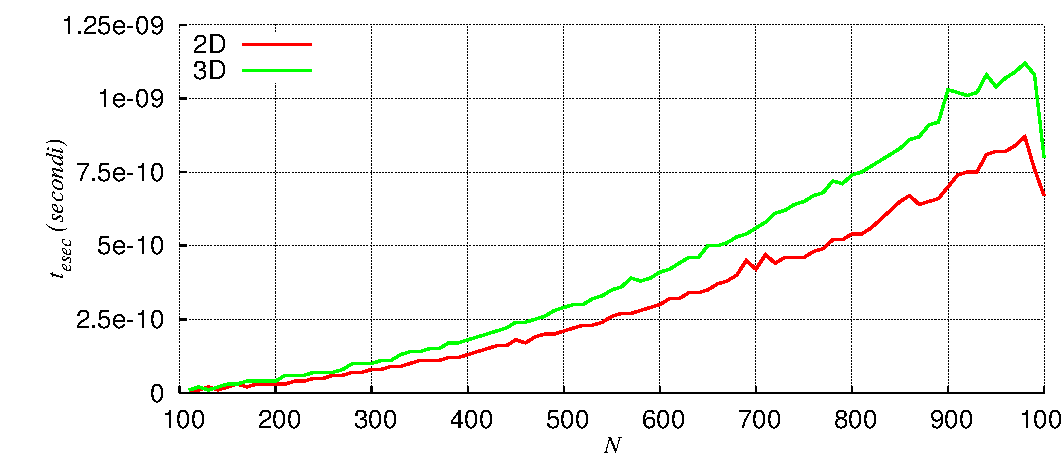
\includegraphics[scale=0.5]{Immagini/Soffici/TempoEsecuzione_ConfrontoD}

		\centering  \footnotesize{$\rho=0.8$ , Media su $ 1000000 $ passi}
	\end{figure}
Chiaramente il tempo macchina aumenta al crescere del numero di particelle della simulazione perchè maggiore è il numero di molecole maggiori sono le coppie di vicini da testare.
Una desità molto alta implica che le particelle siano statisticamente molto vicine tra loro e in media andranno calcolate le forze di interazione su un maggior numero di punti.
La dimensionalità dello spazio influisce invece nel "impaccamento" delle particelle in configurazioni tendenzialmente dense, ad esempio una sfera potrà essere posta a contatto di un maggiore numero di sfere nello spazio piuttosto che vincolando tutte queste sfere ad un piano bidimensionale.
	\begin{figure}
		\centering
		\caption[Sfere Soffici$/$Preliminari\_TempoEsecuzione.cpp]{Confronto tra l'andamento del tempo di esecuzione a vari valori di densità del sistema.}\label{fig: T_Esec_Confronto_rho Soffici}
		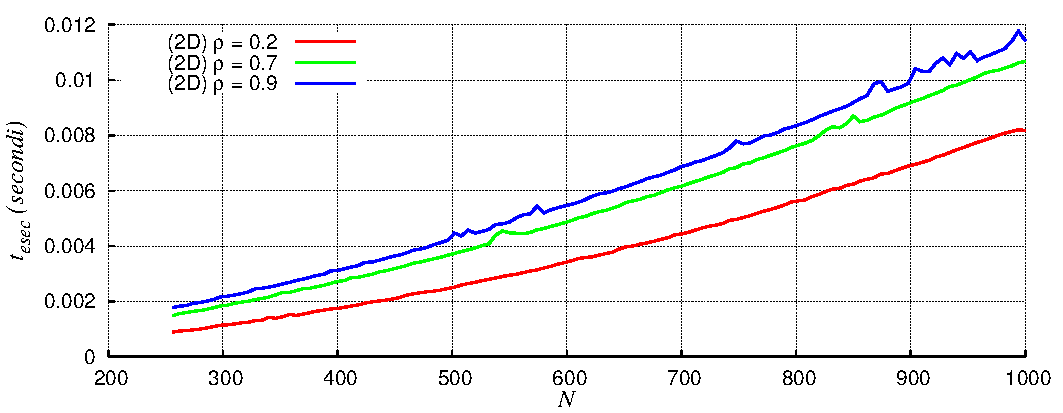
\includegraphics[scale=0.5]{Immagini/Soffici/TempoEsecuzione2D}

		\centering  \footnotesize{$d=2$ , Media su $ 50000 $ passi}
	\end{figure}



\subsubsection{Tempo di Termalizzazione}
In questo sistema è possibile definire due tipi di termalizzazione. Nella prima si interviene fissando l'energia meccanica totale del sistema mentre nella siconda si fissa la temperatura del sistema, quindi solo l'enegia cinetica media.
Siccome le due quantità sono di natura differente, una è puramente istantanea e costantemente conservata mentre l'altra è una quantità che istantaneamente è soggetta a fluttuazioni termiche, lo studio del tempo di termalizzazione va effettuato in modo separato.

	\begin{figure}
		\centering
		\caption[Sfere Soffici$/$Preliminari\_Termalizzazione.cpp]{Andamento degli osservabili istantanei in funzione del numero di passi d'evoluzione per vari valori di densità}\label{fig: Termal E D Soffici}

		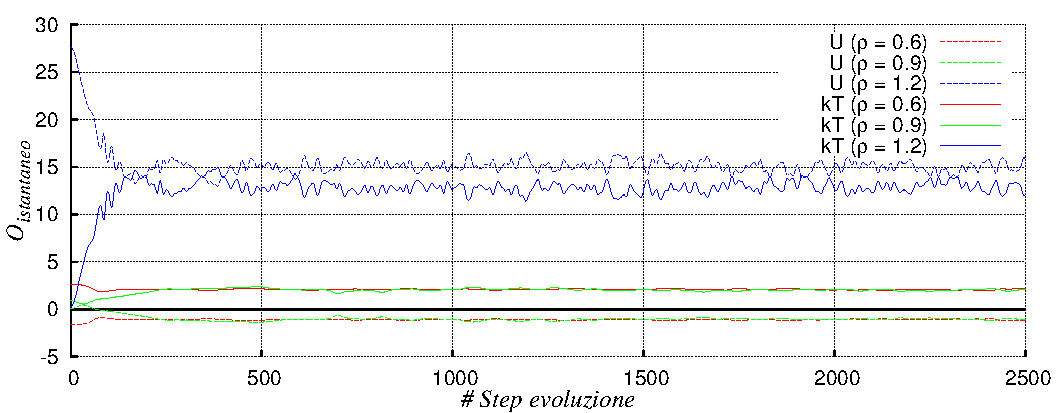
\includegraphics[scale=0.5]{Immagini/Soffici/Termal_OvsStep}

		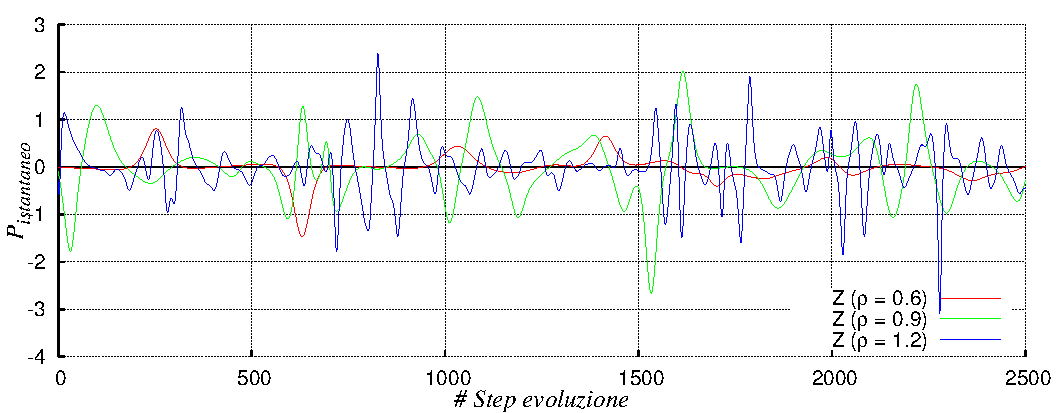
\includegraphics[scale=0.5]{Immagini/Soffici/Termal_PvsStep}

		\centering  \footnotesize{$N= 250$ , $d=3$ , $E_D$ per particella =1}
	\end{figure}
Il tempo di termalizzazione ad Energia definita si può studiare osservando l'andamento degli osservabili istantanei in funzione del numero di step di evoluzione, quando i valori tendono ad oscillare intorno ad un valore medio si può considerare raggiunta la condizione di termalizzazione. 
Secondo la figura (\ref{fig: Termal E D Soffici}) , dove è mostrato l'andamento di $P$,$kT$ e$U$ in funzione del numero di passi di evoluzione, $bubuu$ step sarebbero sufficienti a portare a termalizzazione un sistema di $250$ particelle.
\medskip\newline
Nel caso della termalizzazione a $kT$ definito, invece, si può sfruttare la funzione di $H$ di Boltzman per valutare il tempo di termalizzazione.

	\begin{figure}
		\centering
		\caption[Sfere Soffici$/$Preliminari\_Termalizzazione.cpp]{Andamento dei valori della funzione di Boltzman in funzione del numero di passi d'evoluzione per vari valori di densità}\label{fig: Termal H T_D Soffici}
		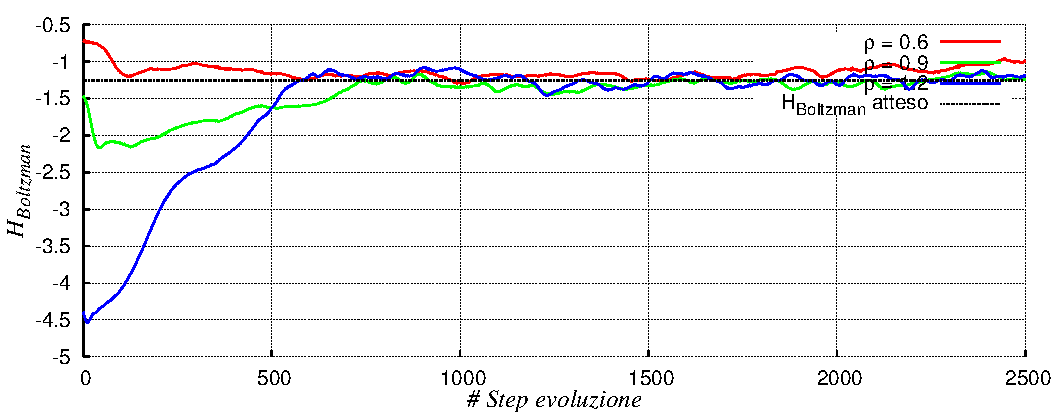
\includegraphics[scale=0.5]{Immagini/Soffici/Termal_HvsStep}

		\centering  \footnotesize{$N= 250$ , $d=3$ , $H$ media calcolata ogni 5 passi}
	\end{figure}
Nella figura (\ref{fig: Termal H T_D Soffici}) è mostrato l'andamento della funzione $H$ calcolata su $25$ configurazioni successive campionate dopo una termalizzazione a temperatura costante ( $kT=1$ ) effettuata per $n$ passi evolutivi a partire dal reticolo $BCC$ iniziale.
Dal grafico si può vedere come i valori campionati comincino ad oscillare attorno al valore atteso dopo circa $1000$ evoluzioni, la statistica presa non è sufficientemente ampia da poter approssimare l'istogramma delle componenti delle velocità alla loro effettiva distribuzione quindi l'accordo completo non si raggiungerà mai.

	\begin{figure}
		\centering
		\caption[Sfere Soffici$/$Preliminari\_Termalizzazione.cpp]{Istogramma della distribuzione dei valori delle componenti x delle velocità raccolte dopo la termalizzazione}\label{fig: Termal Isto T_D Soffici}
		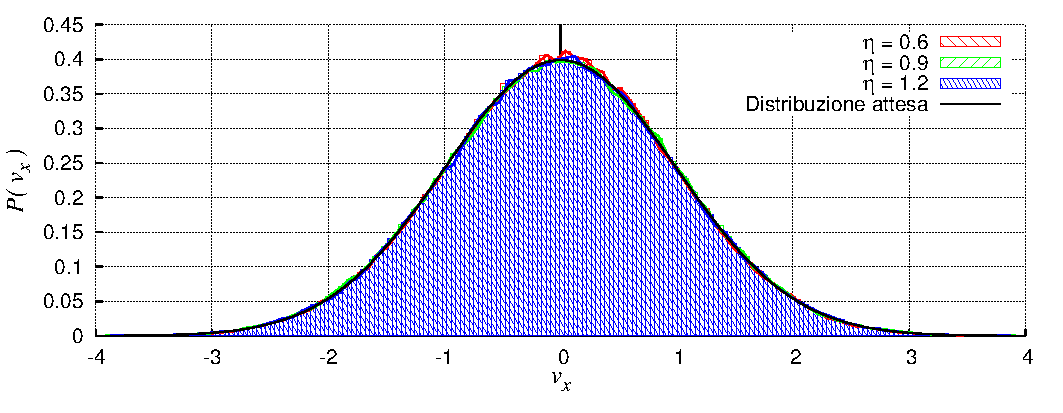
\includegraphics[scale=0.5]{Immagini/Soffici/DistroVx}

		\centering  \footnotesize{$N= 250$ , $d=3$ , N passi Termalizzazione =$ 5000$, $T_D=1$, intervallo di campionamento 50 step.}
	\end{figure}
Aumentando il numero di configurazioni campionate risulta, a seguito della termalizzazione precedente, la distribuzione di probabilità visibile in figura (\ref{fig: Termal Isto T_D Soffici}), che mostra un ottimo accordo con la distribuzione gaussiana prevista per la temperatura prescelta.


\clearpage
\subsection{Caratteristiche del modello, studio delle transizioni di fase}
Per effettuare uno studio completo dell'andamento del parametro d'ordine Z (oppure $ds^2$ o il numero medio di vicini) sarebbe necessario costruire un grafico tridimensionale di tale parametro in funzione di due variabili di stato indipendenti come $\rho$ e $T_D$.
Questo metodo è computazionalmente molto lungo, richiederebbe il calcolo di troppi punti per ottenere una buona risoluzione, per questo l'analisi è limitata a solo due assi ortogonali nel piano $\rho-T$.

Nel primo asse viene fissato $\rho$
uno a rho fisso e a temperatura crescente (inizializzo molto denso poi  espando a desità intermedia(metodo allargamento) e poi riscaldo
seconda parte parto a densità intermedia e temperatura alta e raffeddo)
altro a Temperatura fissa e rho crescente ( solo uno, parto da rho alta e diminuisco gradualmente(con metodo allargamento) termalizzando sempre

\subsubsection{Andamento delle Oscillazioni Termiche}

	\begin{figure}
		\centering
		\caption[Sfere Soffici$/$Problema9.cpp]{Andamento dei valori della densità di energia interna istantanea in funzione del tempo di evoluzione a seguito della termalizzazione.}\label{fig: Problema9}

		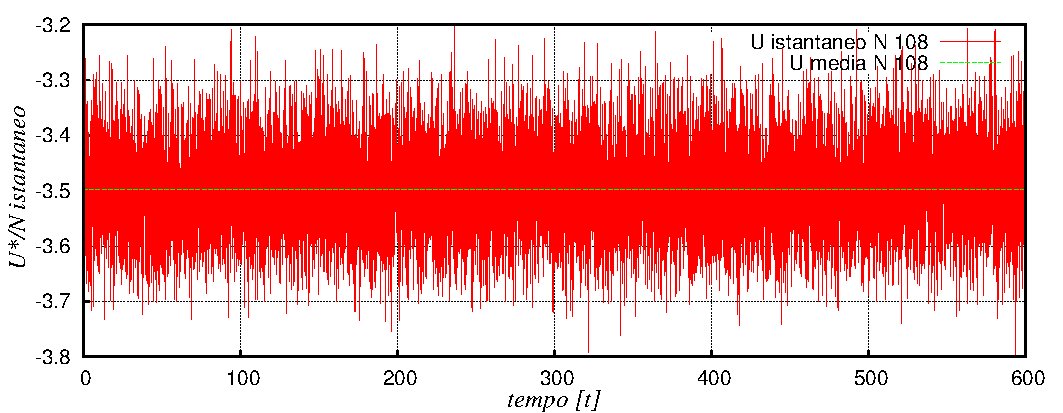
\includegraphics[scale=0.5]{Immagini/Soffici/UvsStepN108}

		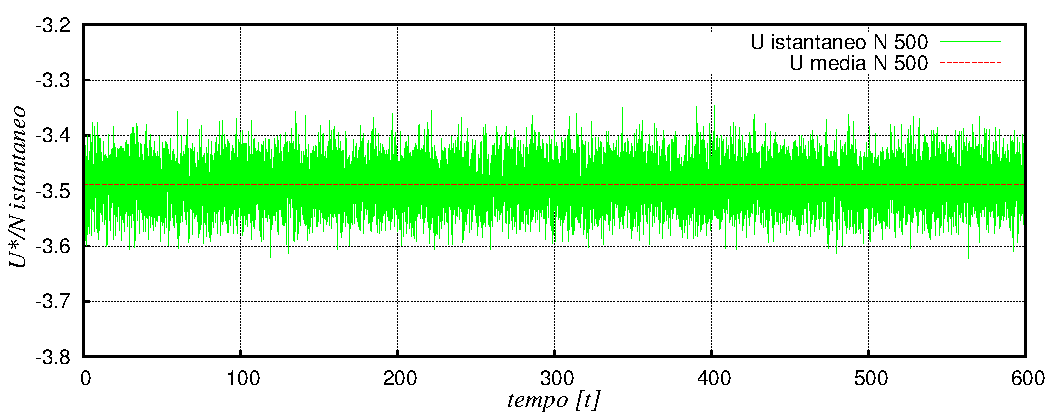
\includegraphics[scale=0.5]{Immagini/Soffici/UvsStepN500}

		\centering  \footnotesize{$N= 250$ , $d=3$ , N passi Termalizzazione =$ 5000$, $\rho = 0.7$,	$T_D=1.19$, campionamento ogni $0.015 [t]$.}

		\caption[Sfere Soffici$/$Problema9.cpp]{Istogramma dei valori campionati per la figura precedente.}\label{fig: Isto_Problema9}

		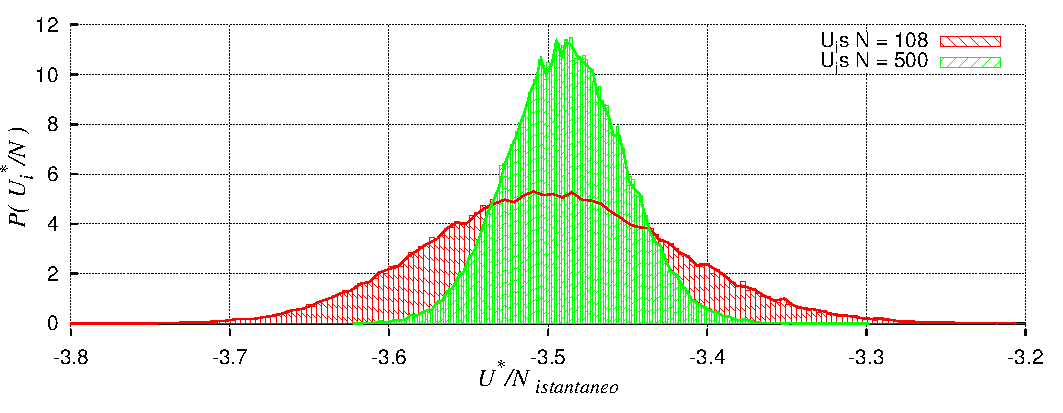
\includegraphics[scale=0.5]{Immagini/Soffici/IstoU}

	\end{figure}
	
	
	\begin{figure}
		\centering
		\caption[Sfere Soffici$/$Problema10.cpp]{Andamento delle osservabili istantanee della simulazione in funzione funzione del tempo di evoluzione a seguito della termalizzazione.}\label{fig: Problema10}
		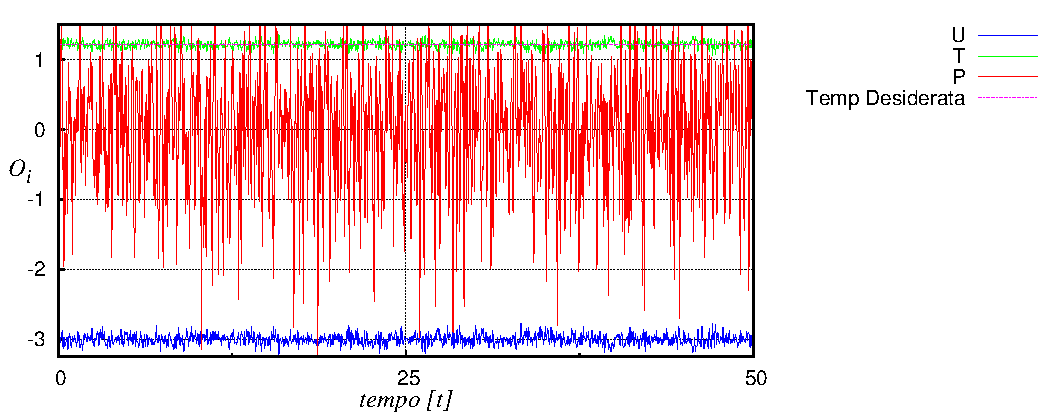
\includegraphics[scale=0.5]{Immagini/Soffici/OvsStep}

		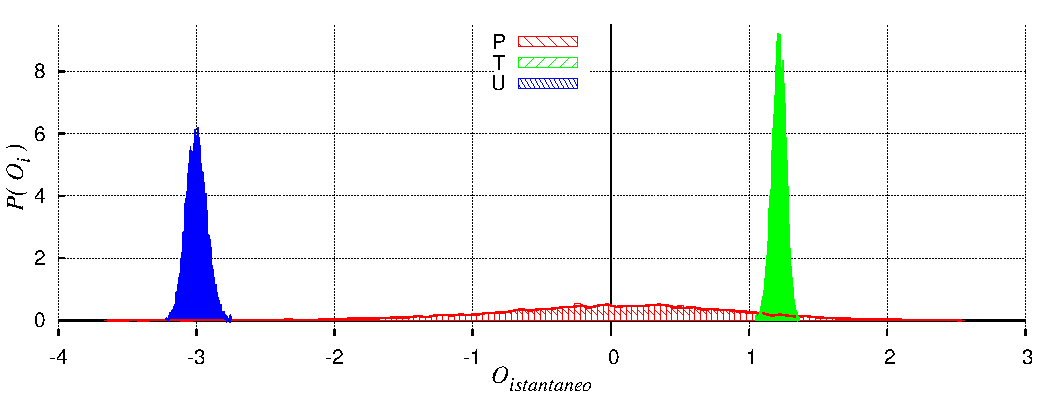
\includegraphics[scale=0.5]{Immagini/Soffici/IstoO}


		\centering  \footnotesize{$N= 108$ , $d=3$ , N passi Termalizzazione =$ 5000$, $\rho = 0.6$,	$T_D=1.22$, campionamento ogni $0.015 [t]$.}
	\end{figure}




\subsubsection{Studio della Diffusione: Spostamento Quadratico Medio.}
	\begin{figure}
		\centering
		\caption[Sfere Soffici$/$Problema11.cpp]{Andamento dello spostamento quadratico medio in funzione del tempo di diffusione per vari valori di temperatura}\label{fig: Problema11}

%		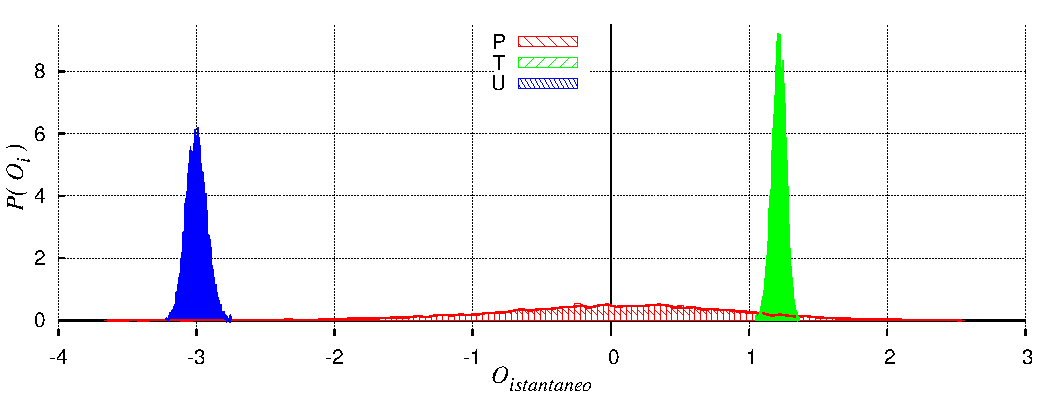
\includegraphics[scale=0.5]{Immagini/Soffici/IstoO}

		\centering  \footnotesize{$N= 256$ , $d=3$ , N passi Termalizzazione =$ 10000$, $\rho = 0.9$, # campionature = $ 4000$, campionamento ogni $0.015 [t]$.}
	\end{figure}



\subsubsection{Studio della Diffusione: Funzione di Distribuzione Radiale}

	\begin{figure}
		\centering
		\caption[Sfere Soffici$/$Problema11_v2.cpp]{Funzione di distribuzione radiale $g_t(r)$ a vari valori di densità e temperatura alta.}\label{fig: Problema11_v2a}

%		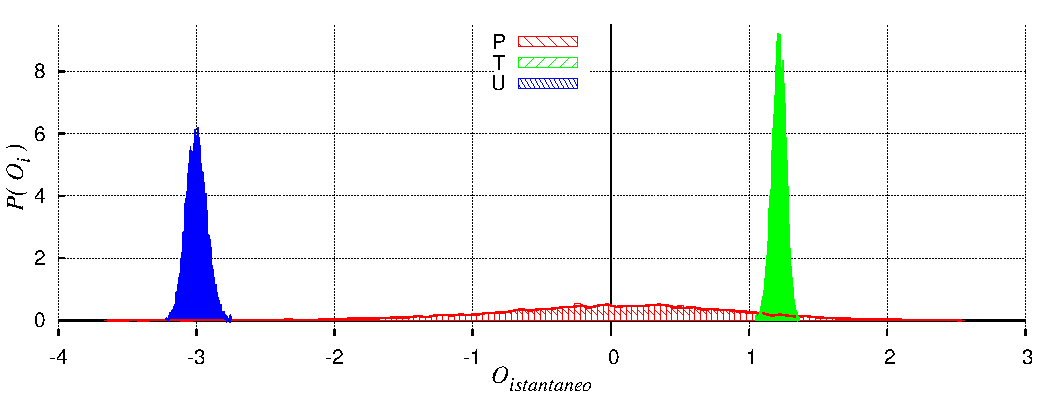
\includegraphics[scale=0.5]{Immagini/Soffici/IstoO}
		\centering  \footnotesize{$N= 256$ , $d=3$ , N passi Termalizzazione =$ 10000$, $\rho = 0.9$, # campionature = $ 4000$, campionamento ogni $0.015 [t]$.}
	\end{figure}

	\begin{figure}
		\centering
		\caption[Sfere Soffici$/$Problema11_v2.cpp]{Funzione di distribuzione radiale $g_t(r)$ a vari valori di temperatura a partire dalla configurazione iniziale congelata.}\label{fig: Problema11_v2b}

%		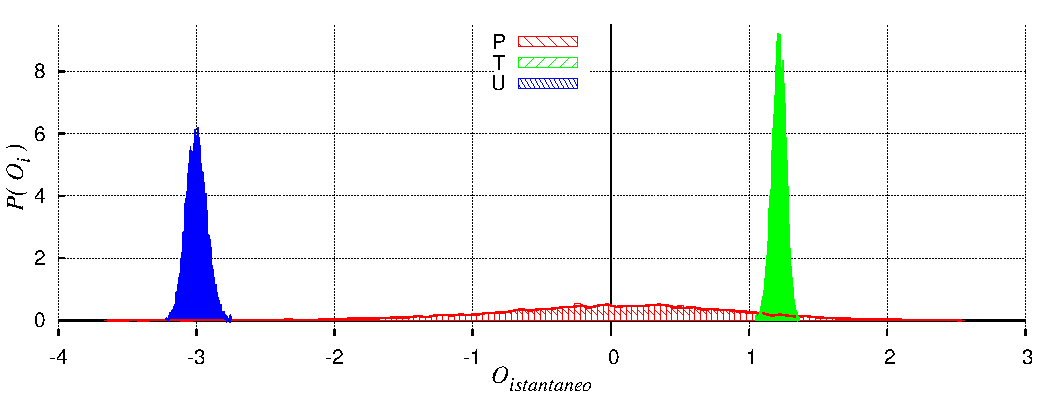
\includegraphics[scale=0.5]{Immagini/Soffici/IstoO}

		\centering  \footnotesize{$N= 256$ , $d=3$ , N passi Termalizzazione =$ 10000$, $\rho = 0.9$, # campionature = $ 4000$, campionamento ogni $0.015 [t]$.}
	\end{figure}


\subsubsection{Studio della relazione tra Temperatura e Energia Meccanica Media.}


\subsubsection{Studio del fattore di comprimibilità come parametro d'ordine}


\clearpage
\subsection{Studio del limite termodinamico}
Nella figura (\ref{fig: Limite Termo}) è mostrato il valore di $\langle Z-1 \rangle$  calcolato per sistemi caratterizzati dalla stessa frazione di impacchettamento ma simulati con diverso numero di particelle.

\begin{figure}[htbp]
\centering
	\caption[Sfere Rigide$/$Problema8.cpp]{Andamento del parametro Z in funzione di $N$. Limite Termodinamico }
%	\includegraphics[scale=0.85]{Immagini/Rigide/ZvsN_3D}
%	\newline\footnotesize{ $d=3$ , campioni$= 500000$,  urti termal=$ 250000$}
	\label{fig: Limite Termo}
\end{figure}
Eseguendo un fit lineare dei valori calcolati risulta:

\begin{displaymath}
 (Z-1) = ()N + ( )
\end{displaymath}
con un $\chi^2$ del ....
Questo permette di stimare un valore del fattore di comprimibilità al limite termodinamico pari a 
\begin{displaymath}
Z_{\textrm{TD}} (\eta = 0.3) = \pm
\end{displaymath}



		\begin{tabbing}
		\emph{microstato.struttura.h} \= definizione della classe microstato \kill
		\emph{microstato.struttura.h} \>\footnotesize definizione della classe microstato \\
		  \>\footnotesize  definizione del costrutture \\
		  \>\footnotesize metodi di inizializzazione  \\
		  \>\footnotesize metodo di flip \\
		\end{tabbing}


\listoffigures

\bibliographystyle{plain}
\bibliography{Bibi.bib}


\end{document}
This is never printed


classi \Cls{Nomeclasse}

metodi \cd{NomeMetodo}

tipo \cd{Nometipo}
